\documentclass[a4paper]{article}
\usepackage{tikz}
\usepackage{ifthen} % Required for conditional checks
\usepackage[margin=1cm]{geometry}  % Ensures correct printable area

\begin{document}
\thispagestyle{empty} % No page numbers

\begin{center}
    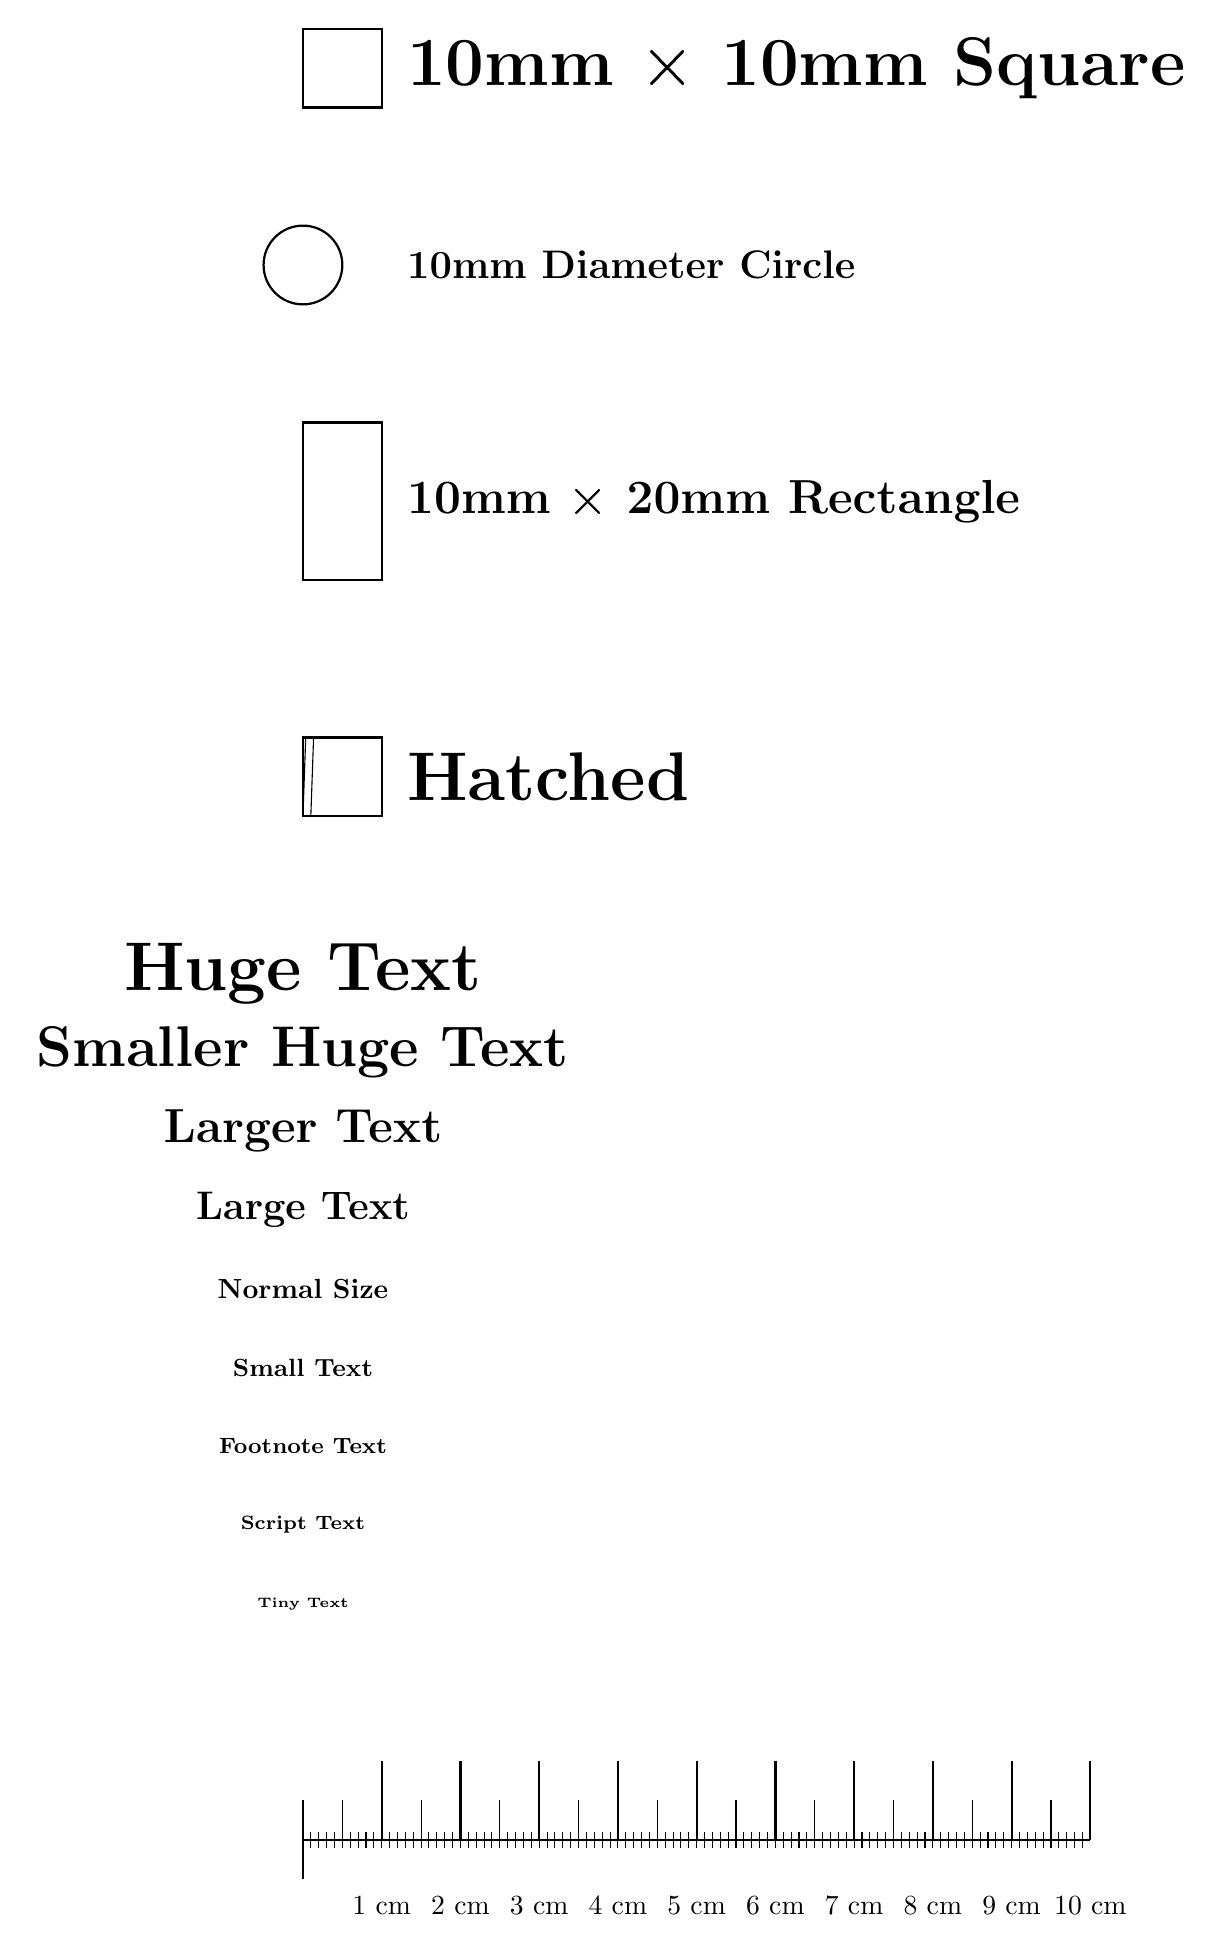
\begin{tikzpicture}
        % === 10mm × 10mm Square ===
        \draw[thick] (0,0) rectangle (1,1);
        \node[right] at (1.2,0.5) {\textbf{\Huge 10mm × 10mm Square}};

        % === 10mm Diameter Circle (Placed Below) ===
        \draw[thick] (0,-2) circle (0.5); % Radius = 5mm (0.5cm)
        \node[right] at (1.2,-2) {\textbf{\Large 10mm Diameter Circle}};

        % === 10mm × 20mm Rectangle (Placed Below) ===
        \draw[thick] (0,-4) rectangle (1,-6); 
        \node[right] at (1.2,-5) {\textbf{\LARGE 10mm × 20mm Rectangle }};

%        % === Angle (L-shape) (Placed Below) ===
%        \draw[thick] (0,-5) -- (0,-6) -- (1,-6); 
%        \node[right] at (1.2,-6.5) {\textbf{\huge Angle (L-shape)}};

        % === Hatched 10mm × 10mm Square ===
        \begin{scope}
            \clip (0,-9) rectangle (1,-8);
            \foreach \x in {-1mm,0mm,1mm,...,10mm} { % Hatch spacing of 1mm
                \draw[thin] (\x,-9) -- (\x+1,-8); % Proper diagonal lines
            }
        \end{scope}
        
        % Draw the border of the square
        \draw[thick] (0,-9) rectangle (1,-8);
        \node[right] at (1.2,-8.5) {\textbf{\Huge Hatched}};



        % === Font Size Examples (Placed Below) ===
        \node at (0,-11) {\textbf{\Huge Huge Text}};
        \node at (0,-12) {\textbf{\huge Smaller Huge Text}};
        \node at (0,-13) {\textbf{\LARGE Larger Text}};
        \node at (0,-14) {\textbf{\Large Large Text}};
        \node at (0,-15) {\textbf{\normalsize Normal Size}};
        \node at (0,-16) {\textbf{\small Small Text}};
        \node at (0,-17) {\textbf{\footnotesize Footnote Text}};
        \node at (0,-18) {\textbf{\scriptsize Script Text}};
        \node at (0,-19) {\textbf{\tiny Tiny Text}};



        % Ruler positioned at (0,-22)
        \begin{scope}[shift={(0,-22)}]
            % Define ruler length (10 cm)
            \def\rulerLength{10} 

            % Draw the main ruler line
            \draw [thick] (0,0) -- (\rulerLength,0);

            % Draw the markings
            \foreach \x in {0,0.1,...,\rulerLength} {
                \pgfmathsetmacro\cmCheck{mod(\x,1)}
                \pgfmathsetmacro\halfCmCheck{mod(\x,0.5)}
                \pgfmathsetmacro\fiveCmCheck{mod(\x,5)}

                % Draw appropriate tick marks
                \ifdim \fiveCmCheck pt = 0pt
                    \draw [thick] (\x,0.5) -- (\x,-0.5); % Every 5 cm
                \else
                    \ifdim \cmCheck pt = 0pt
                        \draw [thick] (\x,0.3) -- (\x,-0.3); % Every cm
                    \else
                        \ifdim \halfCmCheck pt = 0pt
                            \draw [thin] (\x,0.2) -- (\x,-0.2); % Every 0.5 cm
                        \else
                            \draw [thin] (\x,0.1) -- (\x,-0.1); % Every mm
                        \fi
                    \fi
                \fi
            }

            % Big vertical lines every cm
            % Loop for 0.5cm and 1cm marks
            \foreach \x in {0.5,1,1.5,2,2.5,3,3.5,4,4.5,5,5.5,6,6.5,7,7.5,8,8.5,9,9.5,10} {
                \ifthenelse{\equal{\x}{1} \OR \equal{\x}{2} \OR \equal{\x}{3} \OR \equal{\x}{4} \OR \equal{\x}{5} \OR \equal{\x}{6} \OR \equal{\x}{7} \OR \equal{\x}{8} \OR \equal{\x}{9} \OR \equal{\x}{10}}
                { 
                    \draw [thick] (\x,0) -- (\x,1); % Big vertical lines at 1 cm intervals
                    \draw (\x,-0.6) node[anchor=north] {\x\ cm}; % Label for full cm marks
                }
                { 
                    \draw [thin] (\x,0) -- (\x,0.5); % Small vertical lines at 0.5 cm intervals
                }
            }
        \end{scope}

    \end{tikzpicture}


\end{center}

\end{document}
